\documentclass[byrevtex,amssymb,aps,pra,floatfix,letterpaper]{revtex4}
\usepackage{graphicx}
\usepackage{hyperref}
\bibliographystyle{apsrev}
\date{\today}
\pagestyle{plain}

\begin{document}

\title{Experiment 5: IR/Raman spectroscopy and molecular modeling}

\date{\today}

\maketitle

\section{Introduction}
Infrared (IR) and Raman are powerful optical spectroscopy based methods for  detecting vibrational and rotational modes of molecules. In the following, we will concentrate on molecular vibrations and the effect of molecular rotations is discussed elsewhere (see Experiment \#4). Both IR and Raman spectra can be used to identify unknown molecules, determine their concentrations, and to study bond strengths in molecules. For identifying purposes, most spectrometers include a database of IR/Raman spectra and, for small molecules, an on-line database have been compiled \cite{webbook}. Even though both IR and Raman measure molecular vibrations, they are complementary methods for two reasons; they have different selection rules (i.e., some transitions can only be seen in IR whereas others in
Raman) and the requirements for physical characteristics of the samples are different. In this experiment, both IR and Raman methods are applied to determine vibrational frequencies of CCl$_4$, CHCl$_3$, CDCl$_3$ and CH$_2$Cl$_2$ in neat solutions. Molecular rotations are most often quenched in liquids and hence only vibrations will be observed. For an overview of IR and Raman methods, see Refs. \cite{SILBEY,ATKINS1,HERZBERG1,HERZBERG2}. The latter two references also contain an extensive compilation of reference data.

Due to development of modern computers, theoretical methods based on quantum mechanics have become increasingly important tools in modern chemistry. Typically these methods are based on solving of the time-independent Schr\"odinger equation for electrons in atoms or molecules. Among the properties that computational models can predict for the electronic grou\-nd and excited states are: molecular energies and geometries, charge distributions, and various optical and magnetic resonance spectra. In this experiment, the Hartree-Fock method is used to optimize the geometries and predict the vibartional frequencies and IR/Raman intensities of CCl$_4$, CHCl$_3$, CDCl$_3$ and CH$_2$Cl$_2$. The Hartree-Fock method constitutes the lowest level first principles method (``{\it ab initio}''). These results can be compared with the corresponding experimental spectra and assign the peaks to specific
normal modes.

\section{IR and Raman spectroscopy}

For a description of the quantum mechanical harmonic oscillator in the context of molecular vibrations, see Experiment \#4. Here we consider vibration spectra of molecules with multiple bonds by using the normal mode analysis within the harmonic approximation. Recall that the vibrational energy levels in a chemical bond are quantized and that electromagnetic radiation can be used to introduce transitions between the levels (see Fig. \ref{fig1}). The main difference to a diatomic molecule is that, instead of just one bond exhibiting vibrations, now many bonds may participate in the vibrations. Usually the vibrations do not directly correspond to individual bonds but to collective vibrations involving many bonds. These are called the normal modes and their frequencies as well as the participating bonds can be calculated theoretically by diagonalizing the nuclear Hessian matrix \cite{ATKINS2}. For a linear molecule the number of normal modes is $3n - 5$ whereas for non-linear molecules this is $3n - 6$, where n is the number of atoms in the molecule. For example, for HCl (Experiment \#9) we have just one normal mode whereas for H$_2$O we have 3 normal modes. To obtain qualitative understanding of normal modes, consider the normal modes of 
H$_2$O shown in Fig. \ref{fig2}.

\begin{figure}[!htp]
\begin{center}
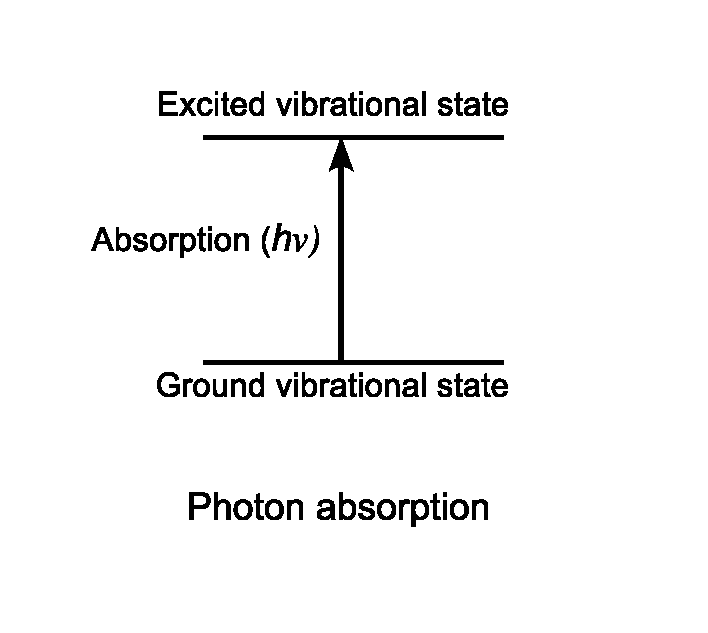
\includegraphics[scale=0.5]{fig1a}
\end{center}
\vspace{-1cm}
\begin{center}
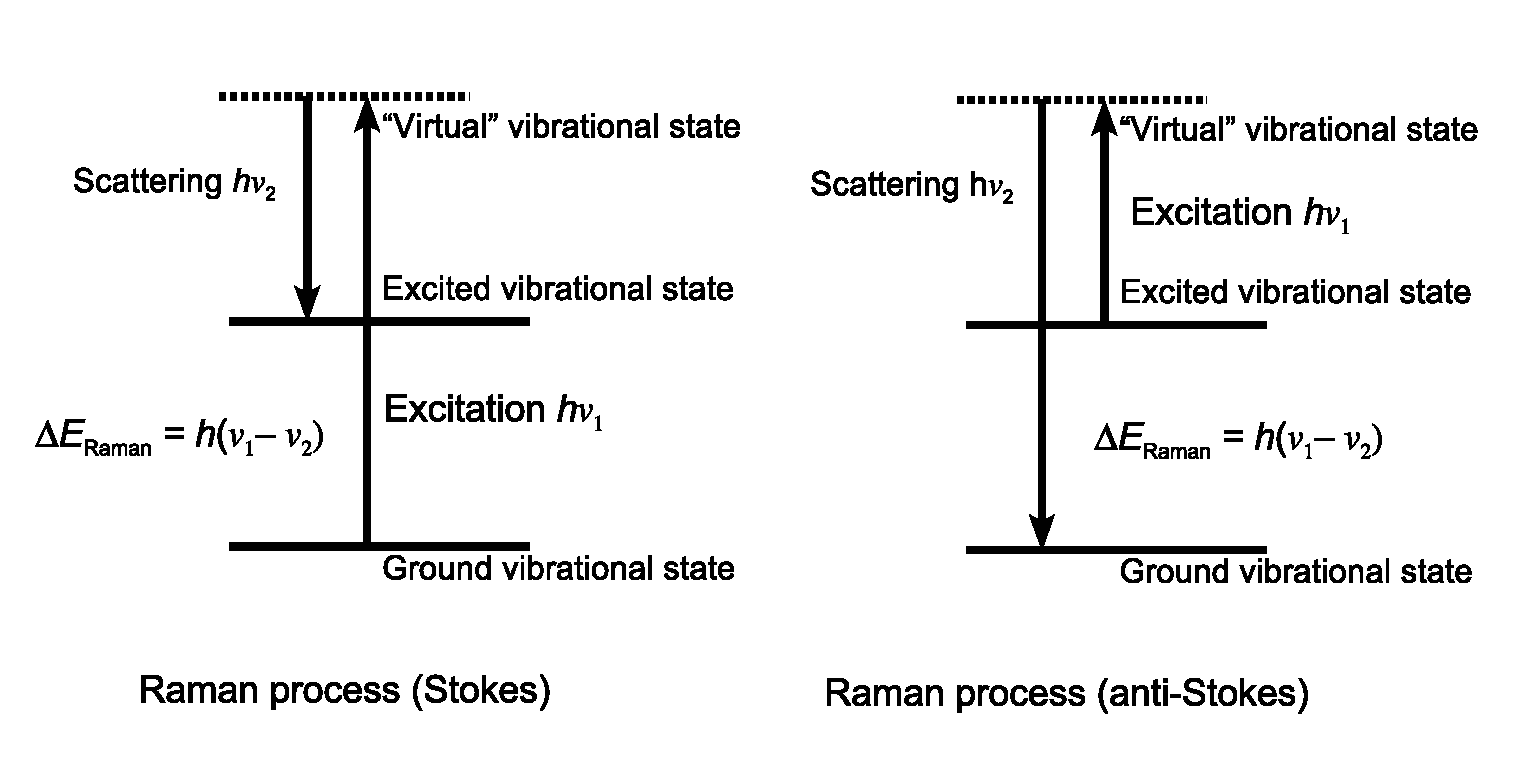
\includegraphics[scale=0.5]{fig1b}
\caption{A schematic description of photon absorption (IR) and Raman processes. A Raman process may proceed under non-resonant condition (``virtual state'') whereas absorption requires resonance. The efficiency of a Raman process is greatly enhanced under resonance conditions. A thermal population of vibrational states is required for anti-Stokes excitation.}
\label{fig1}
\end{center}
\end{figure}

\begin{figure}[!htp]
\begin{center}
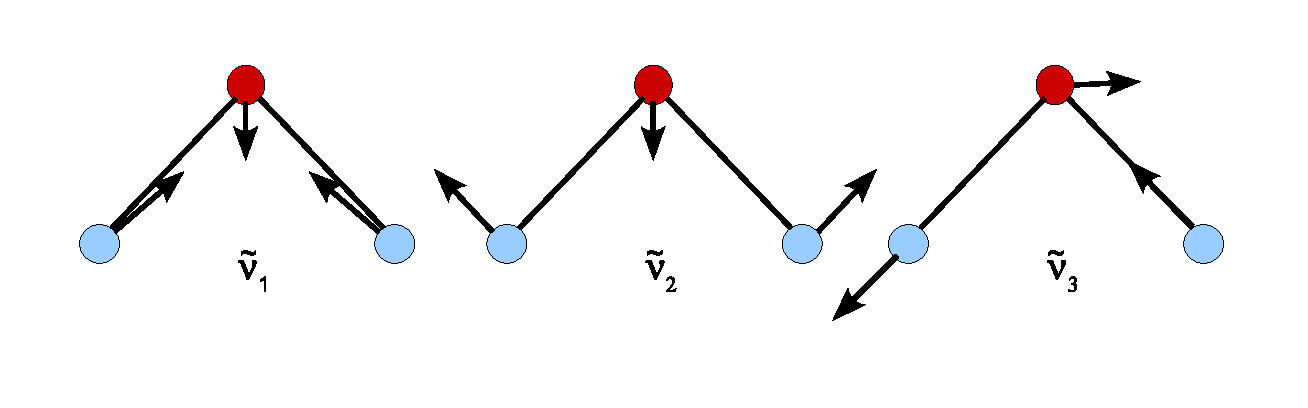
\includegraphics[angle=0, width=10cm]{fig2}
\caption{Normal modes of H$_2$O. The arrows show the direction of the nuclear motion. Note that the ``other direction'' for nuclear motion is obtained when the directions of the arrows are reversed. Note that this method involves the harmonic potential approximation.}
\label{fig2}
\end{center}
\end{figure}

The first mode is called ``symmetric stretch'' ($\tilde{v}_1$), the second ``bend'' ($\tilde{v}_2$) and the third ``asymmetric stretch'' ($\tilde{v}_3$). Each of these modes occurs at a given energy ($\tilde{v}_i$). For example, the transitions shown in Table \ref{table1} have been observed in water vapor. 

\begin{table}[!htp]
\caption{IR bands of water vapor. Note that the energies of the modes are given in the \underline{wavenumber energy units} (cm$^{-1}$) \cite{SILBEY}. The rotational structure is not shown. Fundamental vibrations have been emphasized.}
\begin{tabular}{l@{\extracolsep{2cm}}l@{\extracolsep{2cm}}l@{\extracolsep{2cm}}l}
 & & & \\
$\tilde{v}$ (cm$^{-1}$) & Intensity & Interpretation & Symmetry\\
\textbf{1595.0} & \textbf{Very strong} & $\tilde{v}_2$ & $A_1$\\
3151.4 & Medium strength & $2\tilde{v}_2$ & \\
\textbf{3651.7} & \textbf{Strong} & $\tilde{v}_1$ & $A_1$\\
\textbf{3755.8} & \textbf{Very strong} & $\tilde{v}_3$ & $B_2$\\
5332.0 & Medium strength & $\tilde{v}_2 + \tilde{v}_3$ & \\
6874.0 & Weak & $2\tilde{v}_2 + \tilde{v}_3$ & \\
\end{tabular}
\label{table1}
\end{table}

\noindent
Note that some of the modes in Table \ref{table1} correspond to simultaneous excitation of more than one normal mode. For example, $\tilde{v}_2$ is called an overtone and $\tilde{v}_2 + \tilde{v}_3$ is called a combination vibration. The symmetry label of a given vibration (irreducible representation or irrep for short) can be determined by performing symmetry operations on the mode according to the appropriate point group. For water the point group is $C_{2v}$ (see Table \ref{table2}). Note that the vibrational frequency depends on nuclear masses, which means that for D$_2$O (deuterated water) the vibrational frequencies would be different from H$_2$O. The numbers shown in the table indicate the behavior of a normal mode when a symmetry operator acts on it. A value of 1 means that the mode did not change in the operation and $-1$ indicates that the mode changed the parity in the operation (i.e., directions of the arrows in Fig. \ref{fig2} were reversed). For example, consider the $\tilde{v}_3$ vibration of H$_2$O as shown in Fig. \ref{fig2}. Operation by the identity operator $E$ does not do anything, which means that we get 1. Both operations $C_2$ and $\sigma_{v}(xz)$ exchange the places of the hydrogen atoms and reverses the directions of the arrows in Fig. \ref{fig2}, hence we get $-1$ for both operations. The last symmetry operator $\sigma_{v}'(yz)$ places the mirror plane along the molecular plane and as such does not introduce any changes in the molecule and we get 1. The combination 1, $-1$, $-1$, 1 corresponds to irrep $B_2$ in Table \ref{table1}. Character tables for $C_{3v}$ and $T_d$ groups are given Tables \ref{table3} and \ref{table4}, respectively. Note that two new cases appear as the character may have other values than 1 and $-1$. For example, in $C_{3v}$ the $E$ irreducible representation, which contains two separate degenerate (i.e., the same energy) modes, the identity operation ($E$) includes a sum over both modes: $1 + 1 = 2$. Note that there is an unfortunate use of notation as the symbol $E$ is used for two different purposes: the identity symmetry operation $E$ and the name for irreducible representation $E$. A value of zero means, for example, that the modes had characters like $-1 + 1 = 0$. A symbol $T$ is used for cases
when three modes (or states) are degenerate. Note that this same methodology can be used in working with molecular orbitals. For an overview of molecular symmetry, see Refs. \cite{SILBEY} and \cite{ATKINS1}. The irreducible representations in a group are objects for which a direct product operation can be defined. For example, a direct product of irreps in a given group can be calculated by using the corresponding direct product table for that group. Direct product tables for $C_{2v}$, $C_{3v}$ and $T_d$ are given in Tables \ref{table5}, \ref{table6} and \ref{table7}, respectively. 

\begin{table}[htp]
\caption{Character table for $C_{2v}$ point group. Note that the molecule is taken to reside in the $yz$-plane with $z$ being the main symmetry axis. Here $T$ denotes translation and $R$ rotation along a given coordinate axis.}
\begin{tabular}{l|@{\extracolsep{1cm}}r@{\extracolsep{1cm}}r@{\extracolsep{1cm}}r@{\extracolsep{1cm}}r@{\extracolsep{1cm}}l@{\extracolsep{1cm}}l}
$C_{2v}$ & $E$ & $C_2$ & $\sigma_v (xz)$ & $\sigma_v '(yz)$ & Modes & Operators \\
\hline
$A_1$ & 1 & 1 & 1 & 1 & $T_z$ & $z, x^2, y^2, z^2$ \\
$A_2$ & 1 & 1 & $-1$ & $-1$ & $R_z$ & $xy$ \\
$B_1$ & 1 & $-1$ & 1 & $-1$ & $T_{x}, R_{y}$ & $x, xz$ \\
$B_2$ & 1 & $-1$ & $-1$ & 1 & $T_{y}, R_{x}$ & $y, yz$ \\
\end{tabular}
\label{table2}
\end{table}

\begin{table}
\caption{Character table for $C_{3v}$ point group. The numbers in front of the symmetry operations indicate the number of related operations in that class (for $C_3$ the clockwise and counter-clockwise rotations, for example).}
\begin{tabular}{l|@{\extracolsep{1cm}}r@{\extracolsep{1cm}}r@{\extracolsep{1cm}}r@{\extracolsep{1cm}}l@{\extracolsep{1cm}}l}
$C_{3v}$ & $E$ & $2C_3$ & $3\sigma_3$ & Modes & Operators \\
\hline
$A_1$ & 1 & 1 & 1 & $T_z$ & $z, x^2 + y^2, z^2$ \\
$A_2$ & 1 & 1 & $-1$ & $R_z$ & \\
$E$ & 2 & $-1$ & 0 & $T_{x}, T_{y}, R_{x}, R_{y}$ & $x, y, x^2 - y^2, z^2, xy, xz, yz$ \\
\end{tabular}
\label{table3}
\end{table}

\begin{table}
\caption{Character table for $T_d$ point group.\hfill}
\begin{tabular}{l|@{\extracolsep{1cm}}r@{\extracolsep{1cm}}r@{\extracolsep{1cm}}r@{\extracolsep{1cm}}r@{\extracolsep{1cm}}r@{\extracolsep{1cm}}l@{\extracolsep{1cm}}l}
$T_d$ & $E$ & $8C_3$ & $3C_2$ & $6S_4$ & $6\sigma_d$ & Modes & Operators \\
\hline
$A_1$ & 1 & 1 & 1 & 1 & 1 & & $x^2 + y^2 + z^2$ \\
$A_2$ & 1 & 1 & 1 & $-1$ & $-1$ & & \\
$E$ & 2 & $-1$ & 2 & 0 & 0 & & $ 2z^2-x^2-y^2,x^2-y^2$ \\
$T_1$ & 3 & 0 & $-1$ & 1 & $-1$ & $R_x,R_y,R_z$ & \\
$T_2$ & 3 & 0 & $-1$ & $-1$ & 1 & $T_x,T_y,T_z$ & $x,y,z,xy,xz,yz$ \\
\end{tabular}
\label{table4}
\end{table}

\begin{table}
\caption{Direct product table for $C_{2v}$.\hfill}
\begin{tabular}{l|@{\extracolsep{1cm}}l@{\extracolsep{1cm}}l@{\extracolsep{1cm}}l@{\extracolsep{1cm}}l}
$C_{2v}$ & $A_1$ & $A_2$ & $B_1$ & $B_2$ \\
\hline
$A_1$ & $A_1$ & $A_2$ & $B_1$ & $B_2$ \\
$A_2$ & $A_2$ & $A_1$ & $B_2$ & $B_1$ \\
$B_1$ & $B_1$ & $B_2$ & $A_1$ & $A_2$ \\
$B_2$ & $B_2$ & $B_1$ & $A_2$ & $A_1$ \\
\end{tabular}
\label{table5}
\end{table}

\begin{table}
\caption{Direct product table for $C_{3v}$\hfill}
\begin{tabular}{l|@{\extracolsep{1cm}}l@{\extracolsep{1cm}}l@{\extracolsep{1cm}}l}
 & & & \\
$C_{3v}$ & $A_1$ & $A_2$ & $E$ \\
\hline
$A_1$ & $A_1$ & $A_2$ & $E$ \\
$A_2$ & $A_2$ & $A_1$ & $E$ \\
$E$ & $E$ & $E$ & $A_1+A_2+E$ \\
\end{tabular}
\label{table6}
\end{table}

\begin{table}
\caption{Direct product table for $T_d$.\hfill}
\begin{tabular}{l|@{\extracolsep{1cm}}l@{\extracolsep{1cm}}l@{\extracolsep{1cm}}l@{\extracolsep{1cm}}l@{\extracolsep{1cm}}l}
 & & & & & \\
$T_d$ & $A_1$ & $A_2$ & $E$ & $T_1$ & $T_2$ \\
\hline
$A_1$ & $A_1$ & $A_2$ & $E$ & $T_1$ & $T_2$ \\
$A_2$ & $A_2$ & $A_1$ & $E$ & $T_2$ & $T_1$ \\
$E$ & $E$ & $E$ & $A_1+A_2+E$ & $T_1+T_2$ & $T_1+T_2$ \\
$T_1$ & $T_1$ & $T_2$ & $T_1+T_2$ & $A_1+E+T_1+T_2$ & $A_2+E+T_1+T_2$ \\
$T_2$ & $T_2$ & $T_1$ & $T_1+T_2$ & $A_2+E+T_1+T_2$ & $A_1+E+T_1+T_2$ \\
\end{tabular}
\label{table7}
\end{table}

Group theory is a powerful method for determining the allowed transitions (``selection rules'') in optical spectra. Here we will consider the selection rules for IR and Raman spectra. Intensity of a given transition is proportional
to square of the transition moment (the Fermi Golden rule):
\begin{equation}
\label{eq1}
I\propto \left|\langle\psi_i|H_1|\psi_f\rangle\right|^2=\left|\int \psi_i^* H_1 \psi_f d\tau\right|^2,
\end{equation}
where $H_1$ is a quantum mechanical operator corresponding to the action of the external oscillating electric field (i.e., here visible or IR light) driving the transition. The initial state $\psi_i$, which here corresponds to the vibrational ground state, is always symmetric (recall solutions to the harmonic oscillator problem) and hence it is totally symmetric, $A_1$. The symmetry of the final state $\psi_f$ is obtained from the symmetry of the normal mode (see Fig. \ref{fig2}). For example, for water $\tilde{v}_3$ mode, the symmetry is $B_2$ as shown in Table \ref{table1}. The operator $H_1$ depends on the measurement (e.g., IR or Raman). In IR we consider electron dipole transitions and hence $H_1$ is proportional to operators $x$, $y$, and $z$ (``dipole moment must change in an IR transition''). A Raman process depends on the polarizability of a molecule and hence $H_1$ can be any of the following operators: $x^2, y^2, z^2, xy, yz,$ or $xz$ (``polarizability must change in a Raman transition''). The symmetries for these operators can be found from Tables \ref{table2}, \ref{table3} and \ref{table4}. According to group theory, the integral in Eq. \ref{eq1} is zero unless the direct product of the symmetries of $\psi_i$, $H_1$ and $\psi_f$ give a totally symmetric irreducible representation (such as $A_1$). If the intensity is zero, this means that the transition cannot be observed and we say that it is forbidden. If it is non-zero, it is possible
to observe the transition and it is said to be an allowed transition. Note that this treatment does not give us the actual intensity but just to see if it is zero or non-zero. Consider, for example, the following question: Is the  
$\tilde{v}_3$ mode in H$_2$O IR active? From Table \ref{table1} ($C_{2v}$), we can see that the symmetry of $\psi_f$ is $B_2$ and $\psi_i$ is $A_1$. In IR H1 can be any of $x$ ($B_1$), $y$ ($B_2$) or $z$ ($A_1$) (see the operator column in Table \ref{table2}) and hence we need to check if any of these components yield any IR activity. Using the $C_{2v}$ direct product table gives:
\begin{eqnarray}
\label{eq2}
& & A_1\times B_1\times B_2 = (A_1\times B_1)\times B_2 = B_1\times B_2 = A_2 \ne A_1 \textnormal{(no contribution)}\nonumber\\
& & A_1\times B_2\times B_2 = (A_1\times B_2)\times B_2 = B_2\times B_2 = A_1 \textnormal{(contributes)}\\
& & A_1\times A_1\times B_2 = (A_1\times A_1)\times B_1 = B_1\times B_2 = B_2 \ne A_1 \textnormal{(no contribution)}\nonumber
\end{eqnarray}
Thus this mode is IR active. If none of the above direct products had yielded $A_1$, the transition would have been IR forbidden. Note that IR and Raman have different selection rules.

The symmetries of the modes in a given molecule can also be determined using group theory. In the following, we demonstrate the method for H$_2$O. Water has 3 atoms and each atom has three coordinates associated with them ($x, y, z$). Thus the total number of coordinates to describe H$_2$O is 9. As previously noted, the number of normal modes is $3n - 6 = 3$. The remaining 6 modes are related to translation ($T_x, T_y, T_z$) and rotation ($R_x, R_y, R_z$) of the molecule, which are not of interest in vibrational IR and Raman spectroscopy. First we have to calculate the character $\chi$ for each symmetry operation. Consider Fig. \ref{fig3}, where the local coordinate axes for each atom are shown. For each local coordinate axis, the following rules must be used:

\begin{enumerate}
\item If a local coordinate axis is unchanged in the symmetry operation, a value of 1 is added to the character.
\item If a local coordinate axis changed direction in the symmetry operation, a value of $-1$ is added to the character.
\item If any other displacement of the axis follows, no value is added to the character.
\end{enumerate}
\begin{figure}[!htp]
\begin{center}
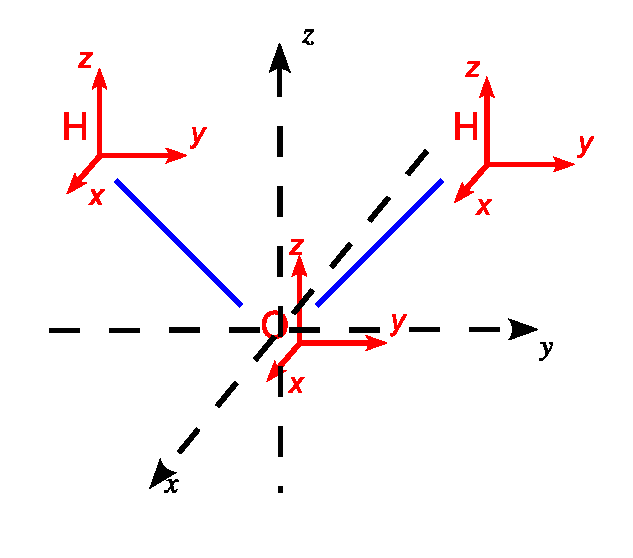
\includegraphics[scale=0.5]{fig3}
\caption{Local coordinates for each atom in H$_2$O are shown. The global coordinate frame for symmetry operations in H$_2$O is also shown.}
\end{center}
\label{fig3}
\end{figure}
For water these rules the characters shown in Eq. \ref{eq3}:

\begin{eqnarray}
\label{eq3}
\chi(E) = 1 + 1 + 1 + 1 + 1 + 1 + 1 + 1 + 1 = 9\nonumber\\
\chi(C_2) = 
\mathop {\overbrace{- 1 - 1 + 1}}\limits^{\textnormal{oxygen}}
\mathop {\overbrace{+ 0 + 0 + 0}}\limits^{\textnormal{hydrogen}}
\mathop {\overbrace{+ 0 + 0 + 0}}\limits^{\textnormal{hydrogen}}
= -1\\
\chi(\sigma_v'(yz)) = 1 + 1 - 1 + 1 + 1 - 1 + 1 + 1 - 1 = 3\nonumber\\
\chi(\sigma_v(xz)) = 1 + 1 - 1 + 0 + 0 + 0 + 0 + 0 + 0 = 1\nonumber
\end{eqnarray}

The next task is to come with irreducible representations that correspond to these characters. First we note that Eq. \ref{eq3} contains both translations and rotations, which from Table \ref{table2} can be seen to correspond to: $A_1$, $A_2$, $2\times B_1$ and $2\times B_2$. Adding these together gives:
\begin{equation}
\label{eq4}
\chi(E) = 6, \chi(C_2) = -2, \chi(\sigma_v'(xz)) = 0 \textnormal{\ and\ }
\chi(\sigma_v(yz)) = 0.
\end{equation}
The only way we can make Eq. \ref{eq3} match with Eq. \ref{eq4} is to add the following irreducible representations to it: $2\times A_1 + B_2$, which correspond to:
\begin{equation}
\label{eq5}
\chi(E) = 3, \chi(C_2) = 1, \chi(\sigma_v'(xz)) = 1 \textnormal{\ and\ }
\chi(\sigma_v(yz)) = 3.
\end{equation}
Thus we conclude that water has three vibrational (fundamental) normal modes, two with $A_1$ symmetry and one with $B_2$ symmetry. This result is in agreement with Table \ref{table1}.

In this experiment, you will study the IR and Raman spectra of CCl$_4$, CHCl$_3$, CDCl$_3$ and CH$_2$Cl$_2$. Based on the above considerations, a table relevant to these compounds can be compiled as shown in Table \ref{table8}.

\begin{table}[!htp]
\caption{Symmetries and IR/Raman activities of vibrational bands. ``IR'' denotes an IR allowed transition and ``R''Raman allowed transition. Note that the table does not say anything about the relative intensities of the lines.}
\begin{tabular}{|l|l|l|l|l|l|l|l|l|l|}
\hline
 & $\tilde{v}_1$ & $\tilde{v}_2$ & $\tilde{v}_3$ & $\tilde{v}_4$ & $\tilde{v}_5$
 & $\tilde{v}_6$ & $\tilde{v}_7$ & $\tilde{v}_8$ & $\tilde{v}_9$\\
\hline
$T_d$ & $E$(R) & $T_2$(IR,R) & $A_1$(R) & $T_2$(IR,R) & -- & -- & -- & -- & --\\
\hline
$C_{3v}$ & $E$(IR,R) & $A_1$(IR,R) & $A_1$(IR,R) & $E$(IR,R) & $E$(IR,R) &
$A_1$(IR,R) & -- & -- & --\\
\hline
$C_{2v}$ & $A_1$(IR,R) & $A_1$(IR,R) & $B_2$(IR,R) & $B_1$(IR,R) & $A_2$(IR,R) &
$B_2$(IR,R) & $A_1$(IR,R) & $A_1$(IR,R) & $B_1$(IR,R)\\
\hline
\end{tabular}
\label{table8}
\end{table}

\section{IR and Raman instrumentation}

Fourier IR and Raman spectrometers are different from the conventional spectrometers, which use dispersive elements (e.g., a grating or a prism). They are based on interference of light in an arrangement called the Michelson interferometer \cite{ATKINS1}. A schematic overview of the spectrometer is shown in Fig. \ref{fig4}. A typical Raman excitation source consists of a continuous wave laser, such as Nd:YAG, which has its fundamental wavelength at 1064 nm. It is important that all the optics in the spectrometer is transparent and the applied detector is sensitive in the wavelength region relevant to the experiment. Transparent regions for some common materials are shown in Table \ref{table9} and detector sensitivity data in Table \ref{table10}. Note that most IR detectors are liquid nitrogen cooled in order to reduce thermal noise. Recall that heat generates IR radiation.

\begin{figure}[!htp]
\begin{center}
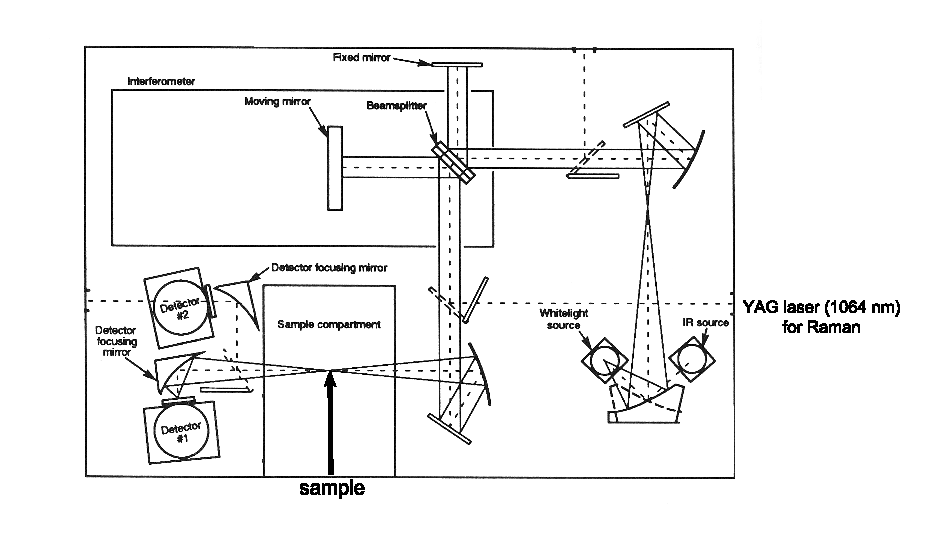
\includegraphics[scale=0.8]{fig4}
\vspace{-1cm}
\caption{A schematic diagram of an FT-IR (including FT-Raman) spectrometer (Nicolet 750). The Raman arrangement involves either a cutoff or notch filter to eliminate the laser (a diode pumped YAG) light from the detector (see Table \ref{table10}). Note that the above setup is explicitly shown for the IR arrangement.}
\label{fig4}
\end{center}
\end{figure}

\begin{table}[!htp]
\caption{Data for optical materials. Materials used in this work have been emphasized.}
\begin{tabular}{l@{\extracolsep{0.5cm}}l@{\extracolsep{0.5cm}}l@{\extracolsep{0.5cm}}l}
Material & Refractive index & Transparent window (cm$^{-1}$) & Optics\\
\textbf{BK-7 glass} & \textbf{1.5} & \textbf{4,300 - 31,000} & \textbf{Sample tube}\\
\textbf{CaF$_2$} & \textbf{1.4} & \textbf{1,300 - 66,000} & \textbf{Beamsplitter}\\
CsBr & 1.7 & 250 - 33,000 & \\
CsI & 1.7 & 150 - 33,000 & \\
Crystal quartz & 1.5 & 3,600 - 50,000 & \\
LiF & 1.3 & 1,500 - 90,000 & \\
\textbf{KBr} & \textbf{1.5} & \textbf{400 - 33,000} & \textbf{Beamsplitter}\\
KCl & 1.5 & 500 - 33,000 & \\
\textbf{NaCl} & \textbf{1.5} & \textbf{700 - 28,000} & \textbf{Sample plates}\\
\end{tabular}
\label{table9}
\end{table}

\begin{table}[!htp]
\caption{Commonly used IR and Raman sensors. Detectors used here are emphasized.}
\begin{tabular}{l@{\extracolsep{2cm}}l@{\extracolsep{2cm}}l@{\extracolsep{2cm}}l}
Detector & Range (cm$^{-1}$) & Detector & Range (cm$^{-1}$)\\
Polyethene & 50 - 650 & MCT-B & 400 - 7,400\\
\textbf{MCT-A} & \textbf{720 - 7,400} & \textbf{InGaAs} & \textbf{5,400 - 11,000}\\
InSb & 1,850 - 10,000 & PbSe & 2,000 - 11,000\\
\end{tabular}
\label{table10}
\end{table}

\section{Experiment}

You will record both IR and Raman spectra of the following neat liquids: CCl$_4$, CHCl$_3$, CDCl$_3$ and CH$_2$Cl$_2$. \textbf{These compounds are toxic - wear gloves and prepare your samples in a hood}. To record an IR spectrum, put two drops of the liquid between two NaCl salt plates and insert the plates into the sample holder inside the FT-IR spectrometer. After measurement, clean the NaCl plates with methylene chloride solution and lens paper. Do not leave fingerprints on the windows. For Raman experiments, pipet a small amount of the sample into a shortened glass NMR tube, install a plastic cap on the tube, and insert the it into the Raman sample holder inside the spectrometer. After measurement, clean the tube with acetone.\\

\noindent
\underline{Measurement of IR spectra}\\

\begin{enumerate}
\item Make sure that the MCT detector has liquid nitrogen in it and that the detector has cooled down. If liquid nitrogen needs to be added, fill a Dewar flask with liquid nitrogen from the tank outside and use the funnel to pour it into the detector (left side of the sample compartment). Handle liquid nitrogen with care and do not spill it on the spectrometer! It is very cold liquid (77 K; $-$196 $^o$C; $-$321 F) and can cause cold burns on your skin. Furthermore, the Dewar flask is made of glass and has vacuum inside the thermally insulated walls, it may explode under rare circumstances and shoot pieces of glass around! \textbf{Wool gloves and a face shield must be worn when handling liquid nitrogen.}

\item \underline{Both the spectrometer and the computer are on at all times}. Ask the instructor to log you in.

\item Make sure that the correct beam splitter is installed (KBr) inside the spectrometer. You can check this by opening the top lid in the spectrometer. If you need to change the beam splitter: turn the handle to release the beam splitter, put it aside into the holder, insert the new beam splitter in place, turn the handle to secure it, and close the lid.

\item If the Omnic program is not running, start it by clicking on its icon on the desktop. Note that the program is often takes long time for the computer to communicate with the spectrometer. Press ``Close'' in the ``Microscopy window'' that comes up first.

\item Make sure that the Raman option (``Use Raman Accessory'') is \underline{unchecked} in the ``Raman'' menu.

\item If measuring the first spectrum, the optical bench inside the spectrometer must be aligned. First remove all samples from the sample compartments. Select ``Collect $\to$ Experimental Setup'', click on ``Bench'' tab. and change detector to MCT/A, Velocity: 1.9, Aperture: 32 and the Gain to 1. Click on the ``Diagnostic'' tab and press ``Align'' button. After the alignment procedure is complete, press ``OK''. This needs to be only once. If the procedure fails, then you may have to click on ``Reset Bench'' and then ``Align''.

\item Select ``Collect $\to$ Experiment Setup''. In the ``Collect'' tab, set the number of scans to 20 and resolution to 2 cm$^{-1}$. Leave the other options as they are.

\item Choose ``Bench'' tab and make sure that the settings are as follows: Sample Compartment: Main, Detector: MCT/A, Beamsplitter: KBr, Source: IR, Accessory: None, Window: None, Max range limit: 4000, Min range limit: 650, Gain: Autogain, Velocity: 1.9, Aperture: 32 and check ``Single beam'' setting box. Finally click ``OK''.

\item Select ``Collect $\to$ Collect sample''. The first spectrum will be the background and you should place just the two NaCl windows in the sample compartment. Click ``OK'' to collect the background (mostly due to H$_2$O vapor and CO$_2$). After the background measurement is done (i.e., ``Sample'' window appears), insert the sample into the IR sample holder inside the spectrometer. Center the sample along the IR beam path, which passes through the center of the sample compartment. Close the sample compartment. If you are unsure where the beam path is located, use a piece of paper to observe the faint red spot from the HeNe laser that is used in aligning the spectrometer. To measure the spectrum, click ``OK'' to collect the sample. After the measurement is done, click ``OK'' to accept the measurement date, click ``Yes'' in the next window to add the spectrum on the screen and finally accept the default window name by pressing ``OK''.

\item Save the spectrum on a USB drive ro a floppy disk by choosing ``File $\to$ Save As''. Change the file type from SPA to CSV, choose the ``A:'' drive, give a filename and hit ``OK''.
\end{enumerate}

\noindent
\underline{Measurement of Raman spectra}\\

\begin{enumerate}
\item \underline{The spectrometer and the computer are on at all times}.

\item Make sure that the correct beam splitter is installed (KBr) inside the spectrometer. You can check this by opening the top lid in the spectrometer. If you need to change the beam splitter: turn the handle to release the beam splitter, put it aside into the holder, insert the new beam splitter in place, turn the handle to secure it, and close the lid.

\item If the Omnic program is not running, start it by clicking on its icon on the desktop. Note that the program is often takes long time for the computer to communicate with the spectrometer. Press ``Close'' in the ``Microscopy window'' that comes up first.

\item Make sure that the Raman option (``Use Raman Accessory'') is \underline{checked} in the ``Raman'' menu and that the IR sample compartment is empty.

\item If measuring the first Raman spectrum, you must align the optical bench inside the spectrometer. This can be done by the following procedure: 1) Turn on the white light source to medium and Gain to 1 in the ``Optical Bench Setup'' dialog, 2) turn the Raman sample holder around to get light reflection from the Raman laser and 4) Press ``Align Bench'' in the ``Optical Bench Setup''. The procedure will take few minutes to complete. After the alignment is done, turn off the white light source, set gain to ``Autogain'' and turn the Raman sample holder back to its original position.

\item Select ``Collect $\to$ Collect Setup''. Set the number of scans to 20 and resolution to 4 cm$^{-1}$. Leave the other options as they are. Accept the changes by clicking ``OK''.

\item Select ``Collect $\to$ Optical Bench Setup''. Make sure that the settings are as follows: Laser ON, Laser Power: 2.0, White light: OFF, Detector: InGaAs, Beamsplitter: KBr, Focus: 70, Aperture: 130, Sample Compartment: Main, check the Spectrum setting box. If measuring the first Raman spectrum, click on ``Quick Align''. If you will not be able to see the spectrum, you may need to come back to this stage and click on ``Align''. For now, click Laser OFF.

\item Insert the sample into the Raman sample compartment (the right side of the spectrometer) and close it.

\item Click on Laser ON and make sure that the laser power is still about 2.0. Finally, click ``OK''. Note: sometimes the laser does not go on (software bug). A workaround for this problem is to turn the white light source on momentarily in the ``Collect $\to$ Optical Bench Setup'' dialog. Remember to turn it off again when you exit the dialog.

\item Select ``Collect $\to$ Collect Raman'' to measure the spectrum. If the display scale is in the range of 9000 cm$^{-1}$, use ``Raman $\to$ Raman Shift'' to get the right $x$-axis scale.

\item Save the spectrum on a floppy disk by choosing ``File $\to$ Save As''. Change the file type from SPA to CSV, choose the ``A:'' drive, give a filename and hit ``OK''.
\end{enumerate}

\noindent
\underline{Finishing up}\\

After all the measurements have been done, make sure that you have cleaned up the NaCl plates (methylene chloride) and the Raman cuvette (acetone). \underline{Make sure that the IR light source and the Raman laser are switched off}:\\

\begin{enumerate}
\item Enter the IR mode by making sure that the ``Use Raman Accessory'' is unchecked in the ``Raman'' menu.

\item Select ``Collect $\to$ Optical Bench Setup'', make sure that the ``Source:'' is set to OFF, and click OK.

\item Enter the Raman mode by making sure that the ``Use Raman Accessory'' is checked in the ``Raman'' menu.

\item Select ``Collect $\to$ Optical Bench Setup'' and make sure the LASER setting is OFF. Click OK.

\item Exit the program by choosing ``File $\to$ Exit''.

\item Turn off the monitor but leave the computer and the spectrometer ON.
\end{enumerate}

\section{Quantum chemistry}

Schr\"odinger equation for a molecule can be written as (nuclei fixed):

\begin{equation}
\label{eq6}
-\frac{\hbar^2}{2m_e}\sum_{i=1}^{n}{\Delta_i\psi_k(r_1,...,r_n)}
+ V(r_1,...,r_n)\psi(r_1,...,r_n) = E_k\psi_k(r_1,...,r_n)
\end{equation}

\noindent
where $m_e$ is the electron mass, $\hbar$ is the Planck's constant ($1.05457148\times 10^{-34}$ Js), $r_i$'s are the positions of the electrons, $n$ is the number of electrons in the molecule, $\Delta_i$ is the Laplacian operator, $V$ is the Coulomb potential including the electron -- electron repulstion and electron -- nuclear attraction as given in Eq. \ref{eq7}, $\psi_k$ is the many-electron wavefunction for state $k$ and $E_k$ is the energy of the molecule in state $k$ \cite{SILBEY,ATKINS1,ATKINS2}. Note that $\psi_k$ no longer a single molecular orbital when more than one electron is present.

\begin{equation}
\label{eq7}
V(r_1,...,r_n) = 
\mathop {\overbrace{\sum_{i<j}^{n}{\frac{e^2}{4\pi \epsilon_0 |r_i - r_j|}}}}
\limits^{\textnormal{\small electron\ -\ electron\ repulsion}}
- \mathop {\overbrace{\sum_{i,j=1}^{n,N}{\frac{eq_j}{4\pi \epsilon_0 |r_i - R_j|}}}}^{\textnormal{\small electron\ -\ nuclear attraction}}
\end{equation}

\noindent
where $N$ is the number of nuclei in the molecule, $q_j$ is the nuclear charge for nucleus $j$, $R_j$ is the position of nucleus $j$, $e$ is the electron charge ($1.6021773 \times 10^{-19}$ C), and $\epsilon_0$ is the vacuum permittivity ($8.8541878 \times 10^{-12}$ As V$^{-1}$m$^{-1}$). For many-electron atoms and molecules orbitals are only approximations and usually follow from neglecting the electron -- electron correlation interaction. A crude model to understand electron -- electron correlation is that the electrons attempt to avoid each other at close distances. Because of this interaction, it is not possible to solve Eq. \ref{eq6} for many-electron systems analytically. Even approximate numerical calculations are very difficult and are usually not able to deal with the electron correlation problem to the full extent. A relatively simple approach for approximately solving Eq. \ref{eq6} is to write the many-electron wavefunction as:

\begin{equation}
\label{eq8}
\psi(r_1,...,r_n) = \frac{1}{\sqrt{n!}}
\left|\begin{array}{cccc}
\phi_1(r_1) & \overline{\phi_1}(r_1) & ... & \overline{\phi_n}(r_1)\\
\phi_1(r_2) & \overline{\phi_1}(r_2) & ... & \overline{\phi_n}(r_2)\\
... & ... & ... & ...\\
\phi_1(r_n) & \overline{\phi_1}(r_n) & ... & \overline{\phi_n}(r_n)\\
\end{array}
\right|
\end{equation}

\noindent
where $\phi_i$'s are functions that we call orbitals (no overbar is $\alpha$; overbar $\beta$ spin). Note that the wavefunction given by Eq. \ref{eq8} is antisymmetric with respect to particle index exchange (i.e., the Pauli principle for fermions). The determinant in Eq. \ref{eq8} is called the Slater determinant. The use of this type of wavefunction in Eq. \ref{eq6} leads to the Hartree-Fock (HF) method, which ignores the electron -- electron correlation \cite{ATKINS2}. The orbitals are typically expressed as a linear combination of Gaussian functions $\chi_j$, which are centered at the nuclei:

\begin{eqnarray}
\label{eq9}
 & & \phi_i(\mathop {\overbrace{x, y, z}}^{\equiv r}) = \sum_{j=1}^{N}{c_{i,j}\chi_j(x,y,z;
\alpha_j,l_x^j,l_y^j,l_z^j,x_0^j,y_0^j,z_0^j)}\\
 & & \chi_j(x,y,z) = (x-x_0^j)^{l_x^j}(y-y_0^j)^{l_y^j}(z-z_0^j)^{l_z^j}
exp(-\alpha_j((x - x_0^j)^2 + (y - y_0^j)^2 + (z - z_0^j)^2))\nonumber
\end{eqnarray}

\noindent
where $c_{i,j}$ are the coefficients to be found by the HF method, $\alpha_j$ (``the extent of the basis function''), $l_x^j$, $l_y^j$ and $l_z^j$  (``angular momenta'') are basis set dependent constants and ($x_0^j$, $y_0^j$, $z_0^j$) are the nuclear coordinates. Actual calculations usually add one more level of sophistication to Eq. \ref{eq9} by grouping Gaussians (``contraction''), but for simplicity, we do not consider it here in detail \cite{ATKINS2}. A group of Gaussians in Eq. \ref{eq9} is called the basis set and is usually denoted by various acronyms like STO-3G, 3-21G, 6-31G*, etc. The larger the basis set is, the higher the accuracy of the calculation will be (in the expense of the computer time). In the HF method, a set of non-linear equations is obtained, which have to be solved numerically by using iterative methods (``self-consistent field method''; SCF). The HF method is often considered as the lowest level method based on the first principles (\textit{ab initio}). Many modern quantum chemistry computer programs like Spartan, Gaussian, Aces-II, Molpro, and GAMESS-US implement the HF method. An input to these programs would typically consist of the nuclear coordinates, the number of electrons (or total charge), the total spin and the symmetry of the molecule. The HF method provides an approximation for the energy of a given nuclear configuration. This energy can be minimized with respect to the nuclear coordinates and results in the minimum energy geometry for a molecule. Such optimization method usually consists of calculations of the energy gradient and iteratively finding the energy minimum by moving the nuclei around. Once the optimum geometry is found, the second derivative matrix of energy can be calculated (``Hessian'') to obtain the normal modes \cite{ATKINS2}.

In this experiment, the HF method with a 3-21G basis set will be employed to calculate the equilibrium geometries and vibrational modes for CCl$_4$, CHCl$_3$ and CH$_2$Cl$_2$ molecules. The Spartan package (commercial) will be used for the HF calculations and to visualize the molecular orbitals and the normal modes.

\section{Calculations using Spartan}

Carry out the RHF/3-21G calculations on CCl$_4$, CHCl$_3$ and CH$_2$Cl$_2$ molecules according to the instructions below. Here RHF = Restricted Hartree-Fock, which is the HF theory for closed shell molecules. For open shell molecules, the unrestricted Hartree-Fock (UHF) theory must be used.

If you haven't created a directory for yourself on the desktop, do it now. Store all your files in this directory. Files that are not stored in appropriate folders will be deleted without a warning! Along the way, you may also want to make printouts (``File $\to$ Print'' in Spartan program). Spartan can be started from the command line by typing spartan or by clicking on the ``colored wheel icon'' on top of the screen. For each molecule you have to carry out the following tasks: (I) Build the molecule; (II) Optimize the geometry of the molecule, record the bond lengths and verify the point group; (III) Calculate the vibrational frequencies; (IV) Characterize each vibrational mode accoding to its harmonic frequency and symmetry; and (V) Compare the calcualted and experimental results (including the IR intensities). Note that Spartan can only calculate IR intensities but not Raman intensities. Therefore the experimental and theoretical Raman intensities cannot be compared. The calculations can be carried out as follows:

\begin{enumerate}
\item \textit{Build the molecule}. Choose a new sketch by choosing ``File $\to$ New''. Create the central carbon atom by choosing the $sp^3$ hybridized carbon from the fragment menu on the right. Add the other atoms by choosing the appropriate atom type from the fragment list and click on the open end bonds on the carbon atom. A new atom appears now in this position. Complete the whole molecule. Note that you can rotate the molecule by holding down the left mouse button while moving the mouse and translate by holding down the right mouse button. Save the molecule in your own directory on the desktop by choosing ``File $\to$ Save As''.

\item \textit{Optimize the geometry, calculate vibrational modes and prepare surface plots}. The first two steps can be combined by choosing ``Setup $\to$ Calculations...'' and then selecting:

\begin{itemize}
\item Calculate: \underline{Eqilibrium geometry} at \underline{ground} state with \underline{Hartree-Fock} \underline{3-21G}.
\item Start From: \underline{Initial} geometry.
\item Subject To: \underline{Symmetry}.
\item Total Charge: \underline{Neutral}.
\item Multiplicity: \underline{Singlet}.
\item Compute: \underline{IR}.
\item Print: \underline{Orbitals \& Energies}, \underline{Vibrational Modes}.
\item Options: (empty).
\end{itemize}

To accept the settings press ``OK''. To precalculate the HOMO orbital plot, choose ``Setup $\to$ Surfaces''. In the ``Surfaces'' window click ``Add'', make the following settings:

\begin{itemize}
\item Surface: \underline{HOMO}.
\item Property: \underline{none}.
\item Resolution: \underline{medium}.
\item IsoValue: (uncheck Fixed).
\end{itemize}

and click OK. Close the ``Surfaces'' window for now (the cross in the upper right hand corner). Start the calculation by choosing ``Setup $\to$ Submit''. Next Spartan will acknowledge that the calculation was started. Finally when the calculation is complete, another acknowledgement window appears. Save the results by choosing ``File $\to$ Save''.

\item \textit{Analysis: bond lengths}. To measure bond length between two atoms, use ``Geometry $\to$ Measure Distance'' selection. Record all bond lengths of the molecule. Use the left mouse button to select any two atoms to read their distance (shown at the bottom right hand corner of the screen).

\item \textit{Analysis: symmetries, vibrational frequencies and IR intensities}. Data for vibrational modes can be accessed by using ``Display $\to$ Spectra'' selection. Make sure that the ``IR'' tab is selected at the top. The list shows all the modes along with their vibrational frequencies (in cm$^{-1}$ units), symmetry, IR intensity and degeneracy factor (i.e., modes with the same energy). Note that the translational and rotational degrees of freedom are not shown in the list. Don't close the window yet, it will be used in the next step.

\item \textit{Analysis: visualization of normal modes}. Visualize the relevant vibrational modes by checking the box next to the vibrational frequency in the ``Spectra'' window. You may need to move the ``Spectra'' window to the side to see the molecule in the main window. It now shows vibrational motion along the direction of the selected normal mode. Note that the amplitude of vibration was chosen arbitrarily and has not physical meaning here. This vibrational motion was shown earlier by using arrows (see Fig. \ref{fig2}).

\item \textit{Analysis: HOMO orbital plot}. To display the HOMO orbital, open the ``Surfaces'' window and check the box on the left side of ``HOMO''. The screen should now contain the molecule with its HOMO orbital overlaid. Colors indicate the sign of the orbital. Note that orbitals depend on three coordinates and therefore we can only visualize ``constant value levels'' on the screen. This essentially gives us the shape of the orbital. Uncheck the box to hide the orbital surface plot.

\end{enumerate}

\section{Written laboratory report}

Follow the general instructions for written laboratory reports. In the  ``Results'' section you must present the following information for each molecule: molecular geometry, molecular symmetry, the total number of molecular vibrations, the number of expected (group theoretical) modes in IR and Raman spectra, the number of experimentally observed modes in IR and Raman spectra, the irreducible representations of the modes, and a comparison of the experimental and theoretical vibrational frequencies. Provide also copies of 
the experimental IR and Raman spectra. Verify that each irrep has the right number of modes in it (see Table \ref{table8}). If some modes were not observed in either IR or Raman spectra, provide an explanation why this is so. Provide  literature values along with your experimental results. Address the following questions:\\

\noindent
1) What is the principal difference between CHCl$_3$ and CDCl$_3$ IR and Raman
spectra?\\
2) What is the reason for this difference?\\
3) For CCl$_4$ provide an explanation what the degenerate HOMOs correspond to.\\
4) Why are the HOMO orbitals degenerate in CCl$_4$?\\

\section{References}

\bibliography{../references}

\end{document}
